%%%%%%%%%%%%%%%%%%%%%%%%%
%% Header for standard beamer presentation
%%
%%  PresentationHeader.tex
%%
%%%%%%%%%%%%%%%%%%%%%%%%%

\documentclass[english,10pt]{beamer}

%%%%%%%%%%%%%%%%%%%%
%% Include general header where common packages are defined
%%%%%%%%%%%%%%%%%%%%



%%%%%%%%%%%%%%%%%%%%%%%%%%
%% TEMPLATES
%%%%%%%%%%%%%%%%%%%%%%%%%%


% Simple Tabular

%\begin{tabular}{ |c|c|c| } 
% \hline
% cell1 & cell2 & cell3 \\ 
% cell4 & cell5 & cell6 \\ 
% cell7 & cell8 & cell9 \\ 
% \hline
%\end{tabular}





%%%%%%%%%%%%%%%%%%%%%%%%%%
%% Packages
%%%%%%%%%%%%%%%%%%%%%%%%%%


% general packages without options
\usepackage{amsmath,amssymb,amsthm,bbm}

% graphics
\usepackage{graphicx,transparent,eso-pic}

% text formatting
\usepackage[document]{ragged2e}
\usepackage{pagecolor,color,ulem,soul}








%%%%%%%%%%%%%%%%%%%%%%%%%%
%% Maths environment
%%%%%%%%%%%%%%%%%%%%%%%%%%

%\newtheorem{theorem}{Theorem}[section]
%\newtheorem{lemma}[theorem]{Lemma}
%\newtheorem{proposition}[theorem]{Proposition}
%\newtheorem{corollary}[theorem]{Corollary}

%\newenvironment{proof}[1][Proof]{\begin{trivlist}
%\item[\hskip \labelsep {\bfseries #1}]}{\end{trivlist}}
%\newenvironment{definition}[1][Definition]{\begin{trivlist}
%\item[\hskip \labelsep {\bfseries #1}]}{\end{trivlist}}
%\newenvironment{example}[1][Example]{\begin{trivlist}
%\item[\hskip \labelsep {\bfseries #1}]}{\end{trivlist}}
%\newenvironment{remark}[1][Remark]{\begin{trivlist}
%\item[\hskip \labelsep {\bfseries #1}]}{\end{trivlist}}

%\newcommand{\qed}{\nobreak \ifvmode \relax \else
%      \ifdim\lastskip<1.5em \hskip-\lastskip
%      \hskip1.5em plus0em minus0.5em \fi \nobreak
%      \vrule height0.75em width0.5em depth0.25em\fi}



%%%%%%%%%%%%%%%%%%%%
%% Idem general commands
%%%%%%%%%%%%%%%%%%%%

%\input{/Users/Juste/Documents/ComplexSystems/CityNetwork/Docs/Headers/GeneralCommands.tex}


\usetheme{Boadilla}

%\setbeamertemplate{footline}[text line]{}
%\setbeamercolor{structure}{fg=purple!50!blue, bg=purple!50!blue}

% cybergeo palette (from Clem server)
% #1C6F91, "#df691a", "#77c5ba", "orange", "#2db92d", "#e1ff2f", "#ff2313", "#bbab61
% redefine palette
\definecolor{cybblue}{HTML}{1C6F91}
\definecolor{cyborange}{HTML}{DF691A}
\definecolor{cybbluegreen}{HTML}{77C5BA}
\definecolor{cybgreen}{HTML}{2DB92D}
\definecolor{cybgreenyellow}{HTML}{E1FF2F}
\definecolor{cybred}{HTML}{FF2313}
\definecolor{cybglaucous}{HTML}{BBAB61}


\setbeamercolor{structure}{fg=cybblue}
\setbeamercolor{footline}{fg=orange, bg=orange}

\setbeamercovered{transparent}


\addtobeamertemplate{title page}{\hspace{-0.4cm}\vspace{-1.5cm}\includegraphics[height=1.2cm,width=1.2\textwidth]{template/bandeau3}\\
}{%
%\begin{textblock*}{150mm}(-1cm,-1.5cm)
%\end{textblock*}
}




\addtobeamertemplate{frametitle}{\hspace{-0.4cm}\vspace{-0.1cm}\includegraphics[height=1.2cm,width=1.2\textwidth]{template/bandeau3}\\
}{%
%\begin{textblock*}{150mm}(-1cm,-1.5cm)
%\end{textblock*}
}



% shortened command for a justified frame
\newcommand{\jframe}[2]{\frame{\frametitle{#1}\justify{#2}}}


\newcommand{\noun}[1]{\textsc{#1}}
\newcommand{\jitem}[1]{\item \begin{justify} #1 \end{justify} \vfill{}}
\newcommand{\sframe}[2]{\frame{\frametitle{#1} #2}}

\DeclareMathOperator{\Cov}{Cov}
\DeclareMathOperator{\Var}{Var}
\DeclareMathOperator{\E}{\mathbb{E}}
\DeclareMathOperator{\Proba}{\mathbb{P}}

\newcommand{\Covb}[2]{\ensuremath{\Cov\!\left[#1,#2\right]}}
\newcommand{\Eb}[1]{\ensuremath{\E\!\left[#1\right]}}
\newcommand{\Pb}[1]{\ensuremath{\Proba\!\left[#1\right]}}
\newcommand{\Varb}[1]{\ensuremath{\Var\!\left[#1\right]}}

% norm
\newcommand{\norm}[1]{\| #1 \|}

\newcommand{\indep}{\rotatebox[origin=c]{90}{$\models$}}


\usepackage{textpos}



%%%%%%%%%%%%%%%%%%%%%
%% Begin doc
%%%%%%%%%%%%%%%%%%%%%

\begin{document}



\title{Cybergeo : Bibliom{\'e}trie indirecte par analyse de r{\'e}seau}


%\author{J.~Raimbault$^{1,2}$}

%\institute{$^{1}$G{\'e}ographie-cit{\'e}s (UMR 8504 CNRS)\\
%$^{2}$LVMT (UMR-T 9403 IFSTTAR)}


\date{R{\'e}union 16/12/2015}


%%%%%%%%%%%%%%%%%%%%%%%%%%%%%%%%
\begin{frame}
\titlepage
\end{frame}

%\begin{frame}
%\tableofcontents
%\end{frame}
%%%%%%%%%%%%%%%%%%%%%%%%%%%%%%%%


%\section{Projects Organization}

%\jframe{Projects Organization}{
%   \includegraphics[width=\textwidth,height=0.8\textheight]{figures/orgaProjects}
%}



\section{Collections des données}


\jframe{Architecture de collecte des donn{\'e}es}{
\includegraphics[width=\textwidth]{figures/archi}
}



\section{Résultats}


\jframe{Caract{\'e}ristiques du r{\'e}seau}{
\textit{418670 Noeuds et 570352 Liens ; Diam{\'e}tre : 9 ; Densit{\'e} : 3.25E-6 ; degré moyen : 2.724284}

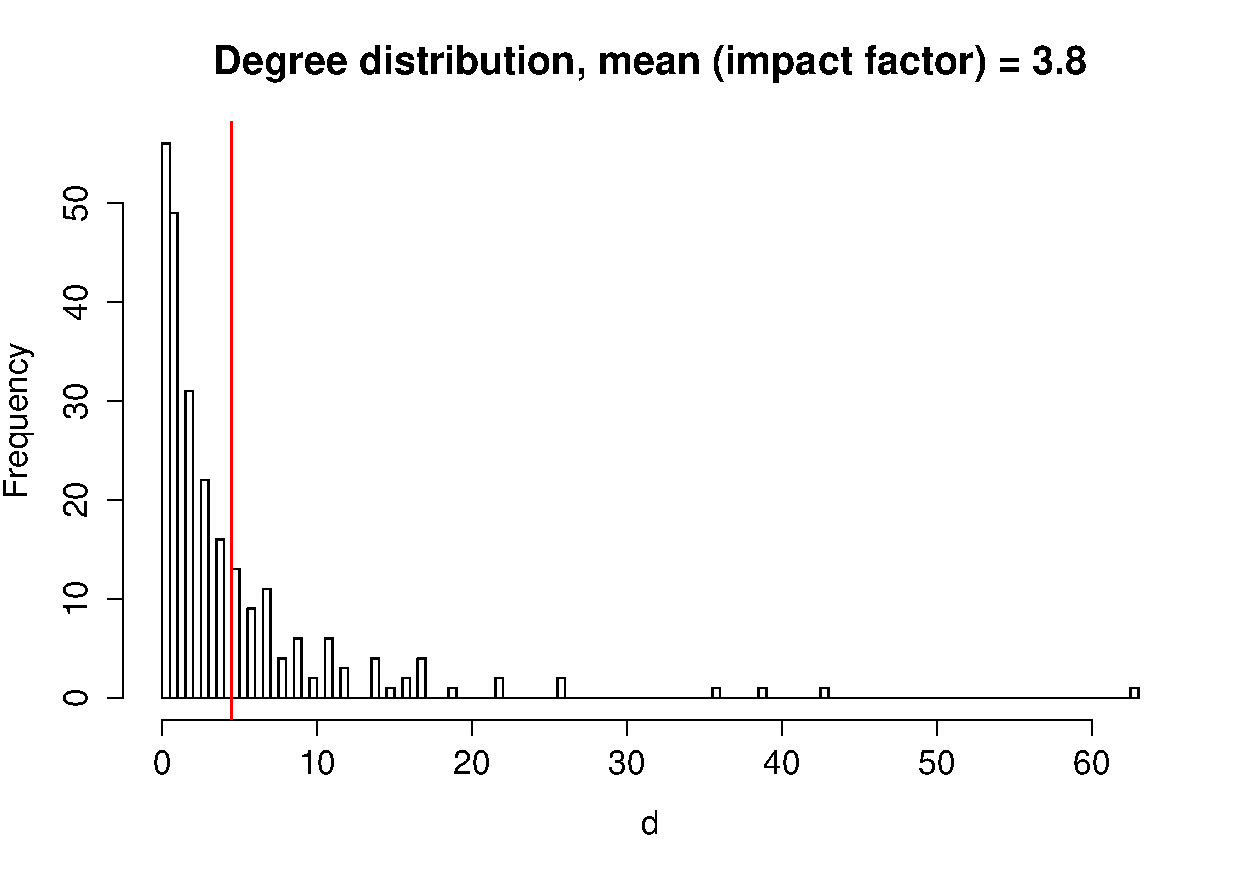
\includegraphics[width=0.8\textwidth]{figures/degreeDistrib}
}

\jframe{Degr{\'e}s : rang-taille}{
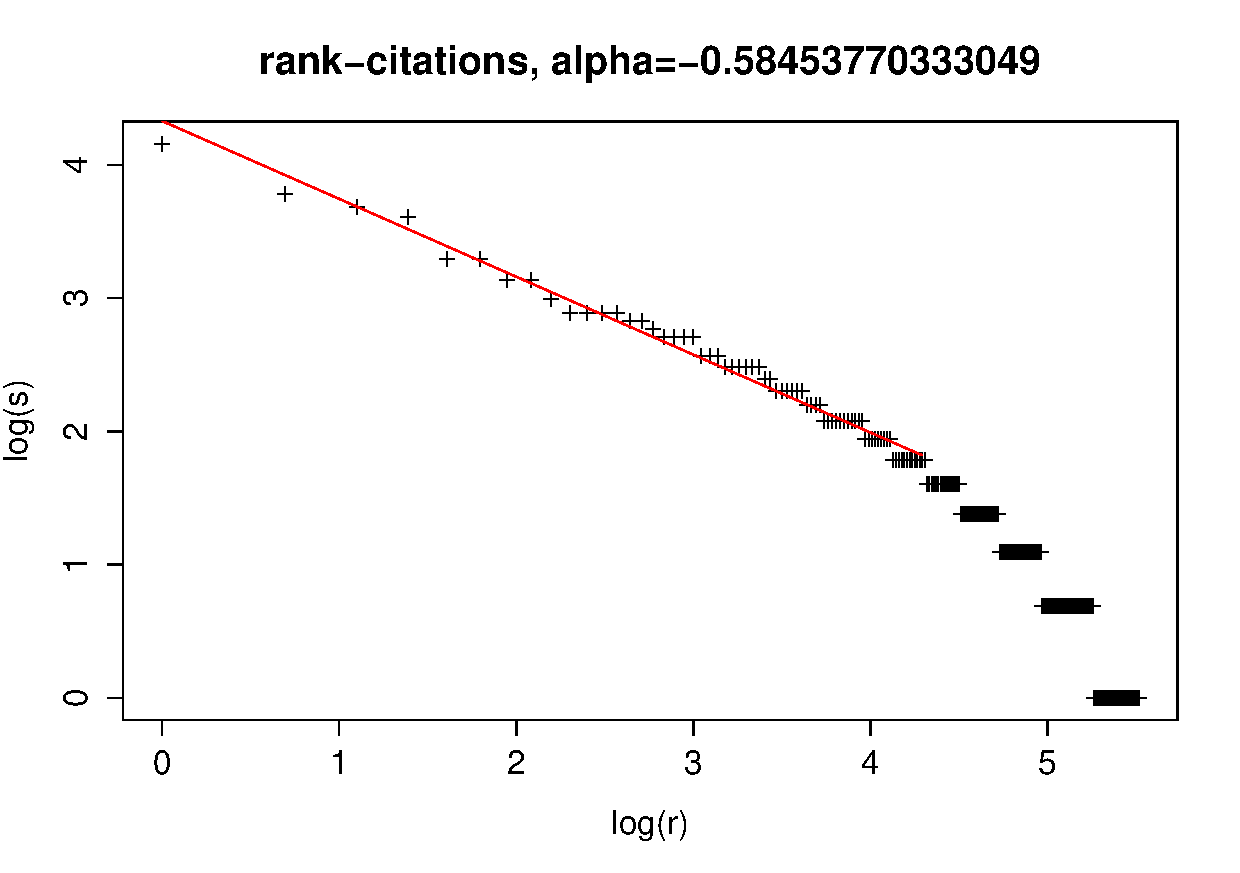
\includegraphics[width=0.52\textwidth]{figures/rankSize_fit}
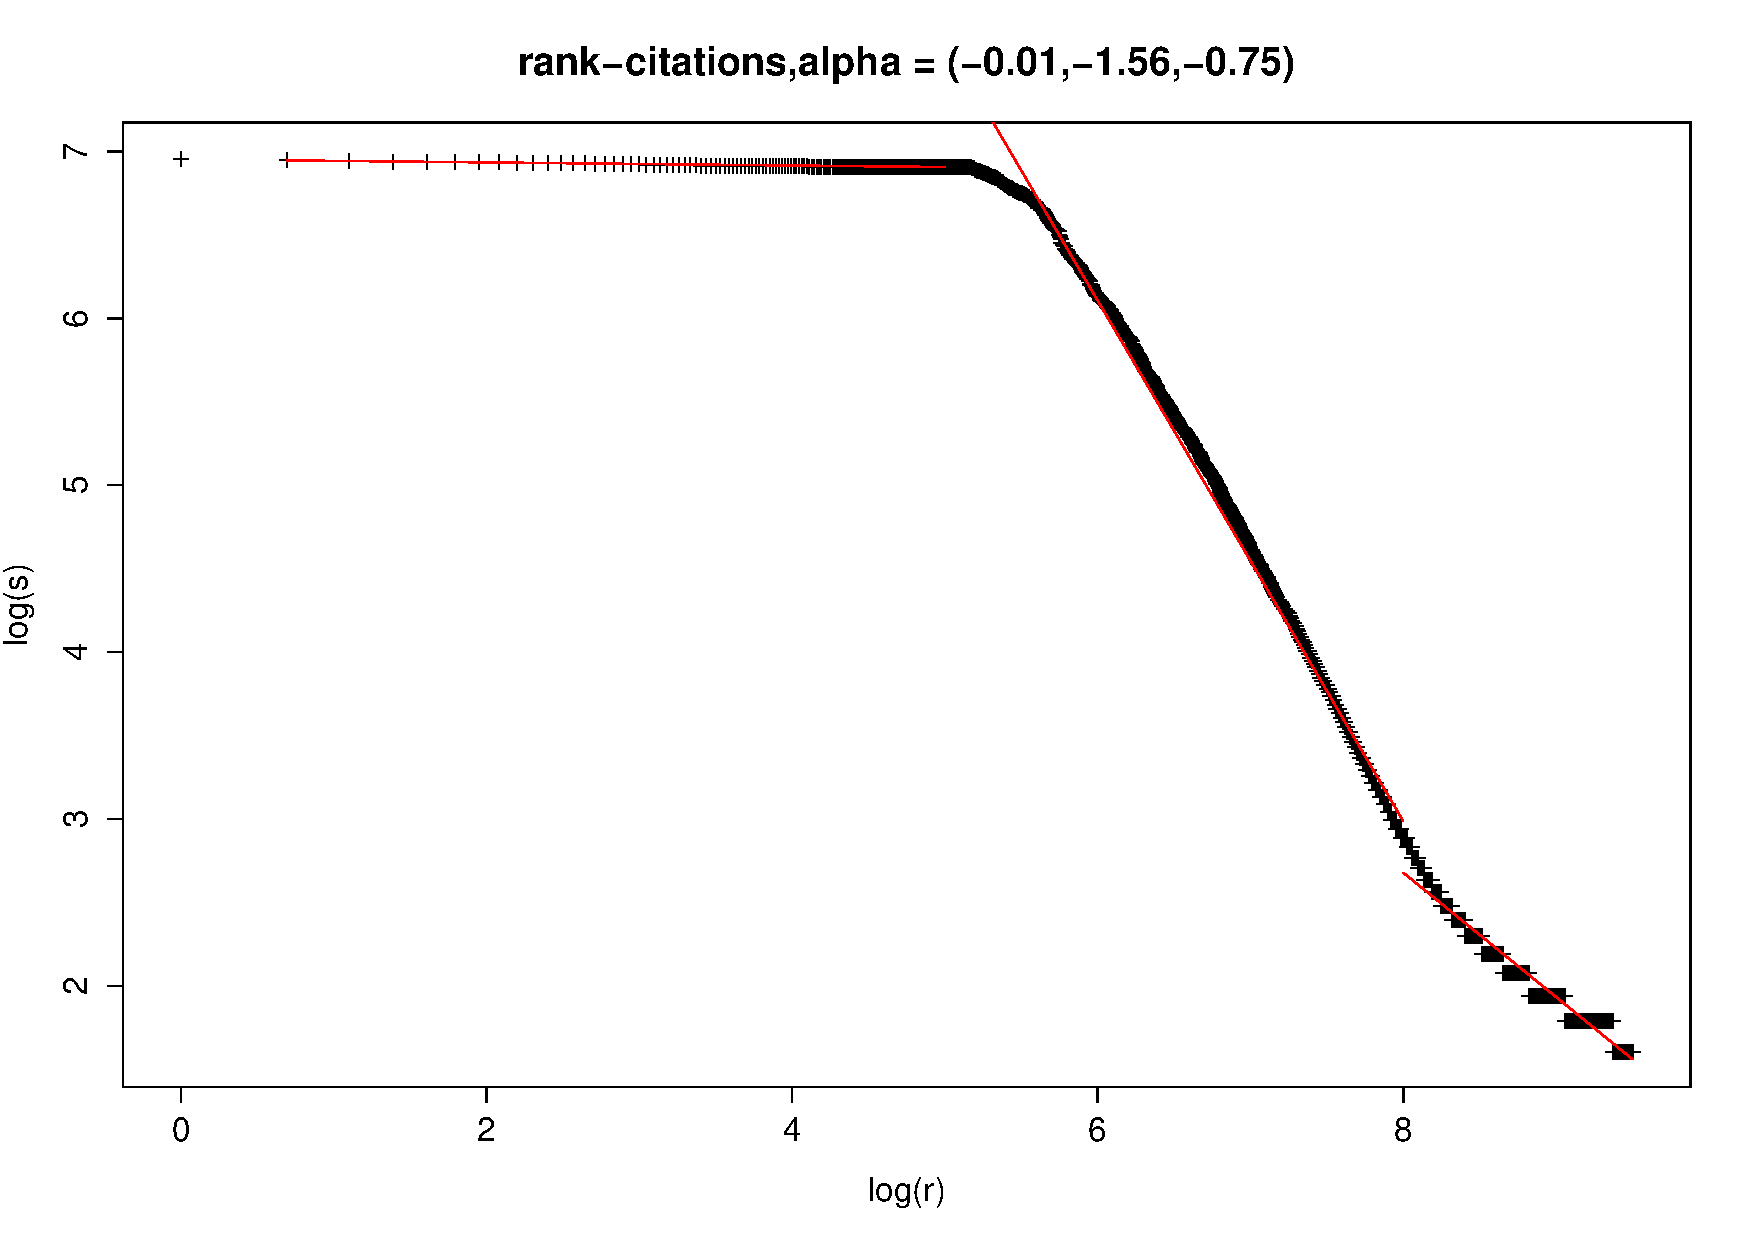
\includegraphics[width=0.5\textwidth]{figures/rank-size-all}

\textit{Gauche : Cyberg{\'e}o ; Droite : Ensemble du r{\'e}seau}

}


\jframe{Clustering}{
Composante g{\'e}ante : plus de 99\% des noeuds.
\medskip

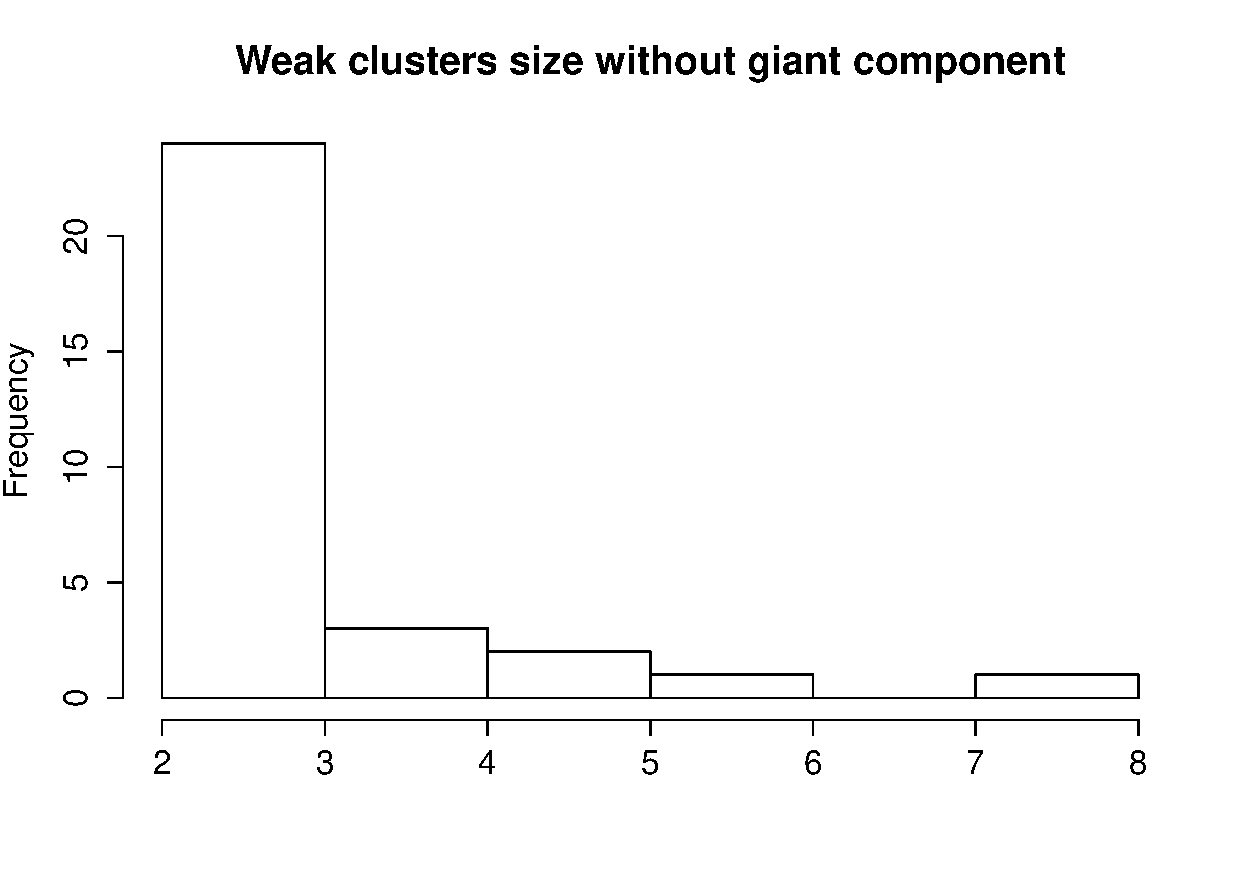
\includegraphics[width=0.5\textwidth]{figures/clusterSize}
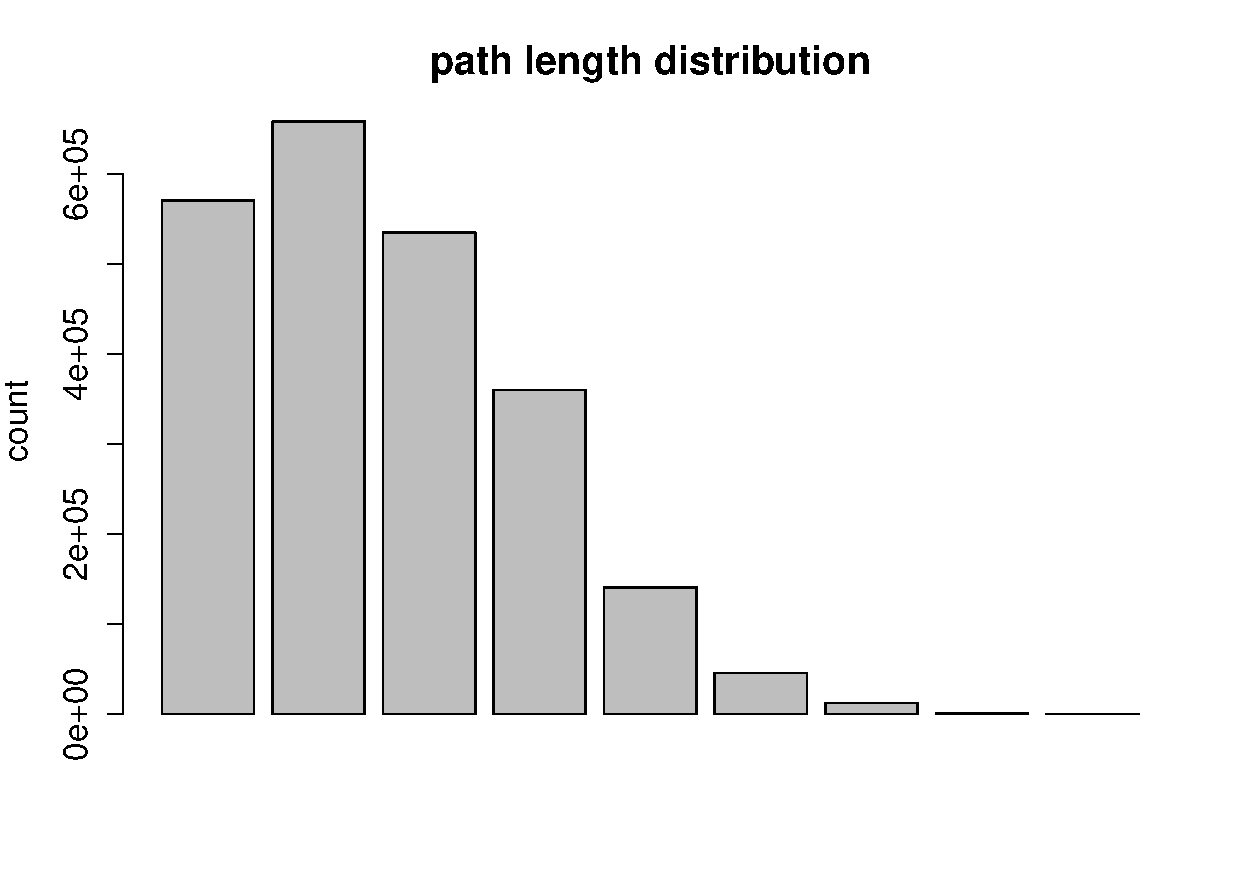
\includegraphics[width=0.5\textwidth]{figures/pathlength}
}



\jframe{Centralit{\'e}}{

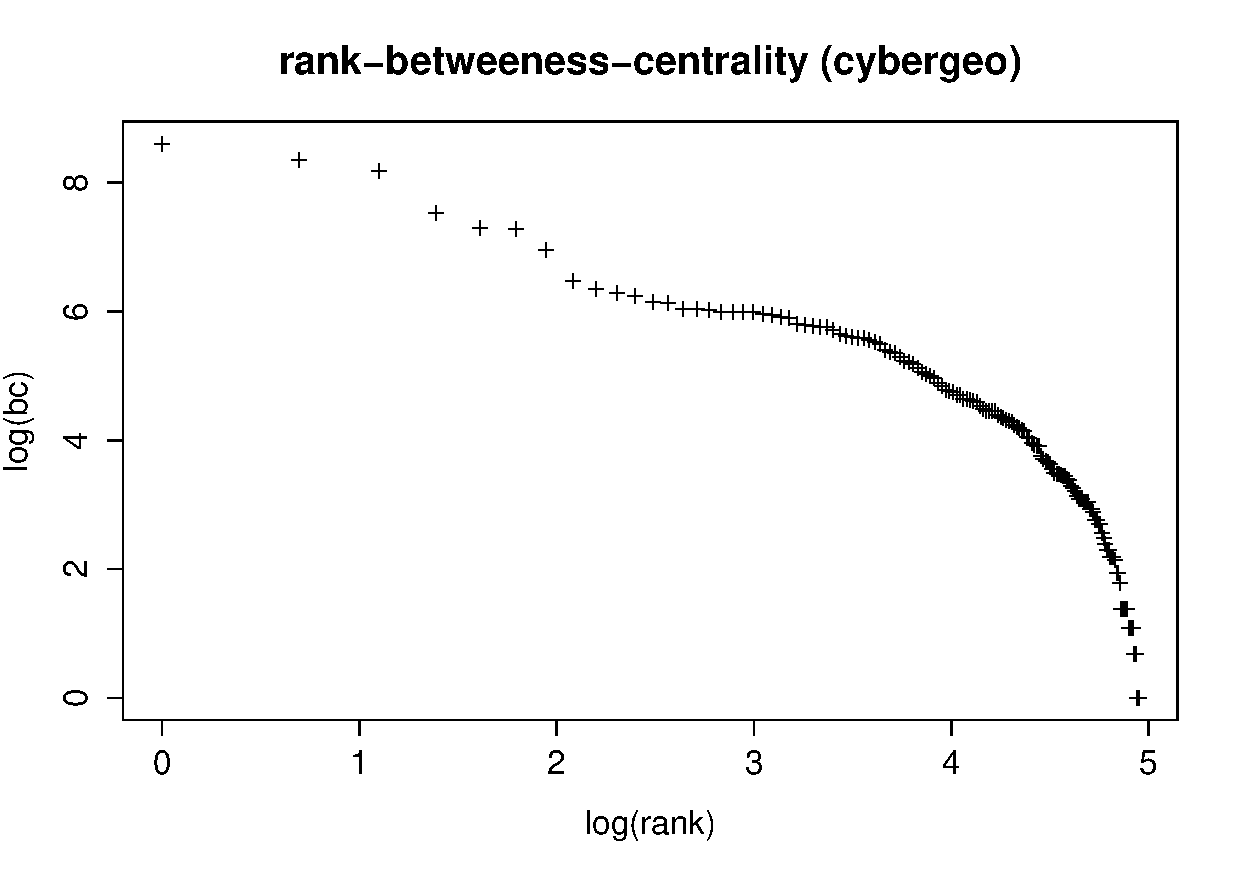
\includegraphics[width=0.5\textwidth]{figures/betweeness-cyb}
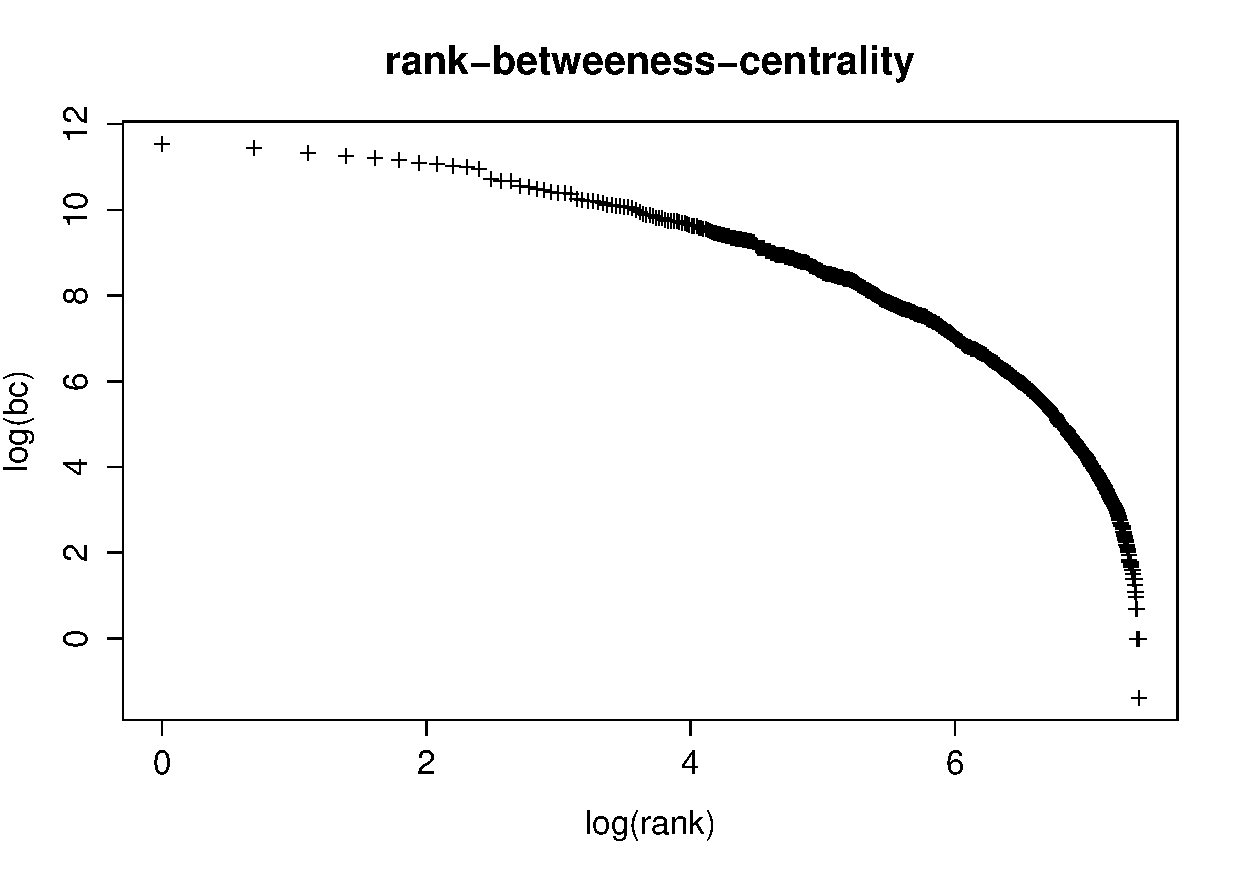
\includegraphics[width=0.5\textwidth]{figures/betweeness}

\textit{Centralit{\'e}s faibles (rq : impossibilit{\'e} des clusters forts pour des citations car causalit{\'e} temporelle). Gauche : Cyberg{\'e}o ; Droite : Ensemble du r{\'e}seau}

}

\section{Suite de l'étude}


\jframe{Suite}{
\begin{itemize}
\item Analyse th{\'e}matique cibl{\'e}e des communaut{\'e}s/cliques
\item Analyses diachroniques
\item Collection des textes des \textit{abstract} pour l'ensemble du corpus
\item Construction du r{\'e}seau s{\'e}mantique ; d{\'e}tection de disciplines par communaut{\'e}s.
\item Croisement des deux couches pour extraire positionnement et importance disciplinaire de cyberg{\'e}o
\end{itemize}

}



\end{document}
